% !TEX TS-program = xelatex
% !TEX encoding = UTF-8 Unicode
% !Mode:: "TeX:UTF-8"

\documentclass{../../styles/resume}
\usepackage{../../styles/zh_CN-Adobefonts_external} % Simplified Chinese Support using external fonts (./fonts/zh_CN-Adobe/)
%\usepackage{../../styles/zh_CN-Adobefonts_internal} % Simplified Chinese Support using system fonts
\usepackage{../../styles/linespacing_fix} % disable extra space before next section
\usepackage{indentfirst}
\usepackage{cite}


\begin{document}

\pagenumbering{gobble} % suppress displaying page number

\begin{center}
  \begin{minipage}{\textwidth}
    \centering
    \name{孟高翔}
    \vspace{0.1em}
    \basicInfo{
      \email{1514190951@qq.com} \textperiodcentered\ 
      \phone{(+86) 136-7557-3771}
    }
    \basicInfo{
      {男 | 武汉大学 | 中共预备党员}
    }
  \end{minipage}
\end{center}

\begin{tikzpicture}[remember picture, overlay]
  \node[anchor=north east, inner sep=0pt] at ([xshift=-1.5cm, yshift=-1.5cm]current page.north east) {
    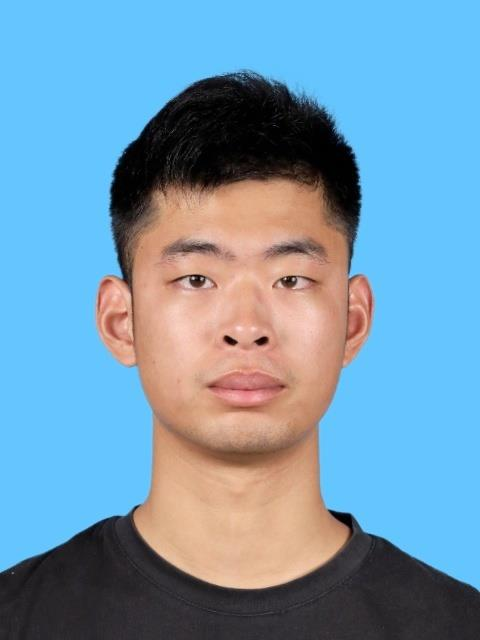
\includegraphics[width=1in]{../../assets/images/photo.jpg}
  };
\end{tikzpicture}

\section{\faGraduationCap\ 教育背景}
\begin{itemize}
  \item \textit{武汉大学计算机学院软件工程}\ 22级本科在读
  \item \textit{GPA:} 3.883/4.0 \quad\quad \textit{排名:} 16/218 (7.339\%)
  \item \textit{主修课程: } 数据结构(92),计算机网络(96),⾼级语⾔程序设计(94),操作系统(91),系统级程序设计(90),数字逻辑与数字电路(90),线性代数(96)
\end{itemize}




\section{\faUsers\ 项目经历}

\datedsubsection{\textbf{财务报销系统}}{2025年3月}
\role{学院项目, 发票内容提取与二维码识别模块开发}{Python, OpenCV}
\begin{onehalfspacing}
开发财务报销系统,实现发票信息自动化提取与处理
\begin{itemize}
  \item 调研技术方案,选用PaddleOCR实现发票文本高效提取与结构化处理
  \item 基于OpenCV与pyzbar开发二维码解析功能,确保高稳定性与准确性
  \item 参与需求分析与系统集成,优化模块性能,提升用户体验
\end{itemize}
\end{onehalfspacing}


\datedsubsection{\textbf{智能招聘匹配平台 (简历匹配)}}{2025年1月}
\role{个人项目}{Python, PyTorch, NLP}
\begin{onehalfspacing}
针对求职痛点(信息冗余、匹配不精准、职位命名混乱),开发智能平台优化求职与招聘体验。
\begin{itemize}
  \item 提取岗位特征(如技能标签、工程阶段),利用BERT模型与DeepSeek API实现自动化特征提取。
  \item 基于Vue.js+ECharts实现行业趋势可视化,辅助求职者洞察市场。
  \item 采用双阶段匹配算法(NER粗排+SentenceTransformer精排),融合规则得分推荐Top 20职位。
\end{itemize}


\end{onehalfspacing}
\datedsubsection{\textbf{Contextual Code Retrieval for Commit Message Generation (C3GEN)}}{2025年4月}
\role{科研项目}{Python, NLP, Static Analysis}
\begin{onehalfspacing}
提出检索增强算法C3GEN,通过从代码检索上下文代码片段结合code diff,生成准确完整的提交信息。
\begin{itemize}
  \item 利用静态语法分析构建代码结构图,包含三类节点及关联关系,并基于code diff增强结构图。
  \item 开发节点建模与去重机制(name-type pair),结合DefinitionIndex提取相关代码片段。
  \item 实现上下文检索与生成流程,提升提交信息质量,实验验证准确率提升约15\%。
\end{itemize}
\end{onehalfspacing}

% \datedsubsection{\textbf{商品数据分析平台}}{2024年6月}
% \role{课程设计, 后端开发/数据处理}{Python, NLP, 数据可视化}
% \begin{onehalfspacing}
% 收集多平台商品数据并进行分析,为用户提供对比数据和情感分析结果
% \begin{itemize}
%   \item 自动爬取多平台商品数据及评论,进行数据清洗与预处理
%   \item 提取评论关键词,生成交互式词云图进行可视化展示
%   \item 利用LDA主题模型对评论进行情感分析,提升分析精准度
% \end{itemize}
% \end{onehalfspacing}

% \datedsubsection{\textbf{大模型终身学习机制研究}}{2025年3月}
% \role{科研项目, 文献调研与技术分析}{Python, Literature Review}
% \begin{onehalfspacing}
% 阅读学习文献,聚焦多模态环境下大模型知识持续更新与遗忘避免
% \begin{itemize}
%   \item 调研10余篇英文学术文献,分析知识更新与模型遗忘技术挑战
%   \item 总结多模态学习关键技术与解决方案
%   \item 积累文献分析与问题抽象经验,提升科研素养
% \end{itemize}
% \end{onehalfspacing}


\section{\faHeartO\ 曾获荣誉}
\datedline{\textit{2024年全国大学生数学建模竞赛 湖北省三等奖}}{2024年09月}
\datedline{\textit{2024年第十五届蓝桥杯大赛C/C++程序设计 湖北省二等奖}}{2024年04月}
\datedline{\textit{2025年中国大学生计算机设计大赛 湖北省三等奖}}{2025年01月}
\datedline{\textit{2024年华为ICT编程赛 湖北省一等奖}}{2024年11月}
\datedline{\textit{2024-2025学年武汉大学优秀学生乙等奖学金}}{2024年10月}


\section{\faInfo\ 个人情况总结}
\begin{itemize}
  \item \textit{英语能力:} 雅思6.5,具备流利听说读写能力,熟练阅读英文学术文献
  \item \textit{技术领域:} 自然语言处理、深度学习、前后端开发、图像处理、语义分析
  \item \textit{综合素质:} 具备扎实数学基础、严谨科研素养、团队协作与创新能力
\end{itemize}


\end{document}
